\documentclass[12pt]{beamer}
\mode<presentation>
\usepackage[utf8]{inputenc}
\usepackage{graphicx}
\usepackage{amssymb,textcomp}
%\usepackage{beamerthemesplit}
\usepackage{beamerthemeBoadilla}
\usefonttheme{serif}
\title{Unidad IV: Diferenciaci\'on e Integraci\'on Num\'erica}
\author{Prof. Jos\'e Luis Ram\'irez}
\date{\today}

\begin{document}

\maketitle

\begin{frame}
  \titlepage
\end{frame}

\begin{frame}{Contenido}
  \tableofcontents
\end{frame}

\section{Introducción}
\begin{frame}{Motivaci\'on}
  El flujo de calor en la interfaz suelo-aire puede calcularse con la ley de Faraday
  \begin{block}{}
    $$
    q = -k\rho C \frac{dT}{dz}
    $$
  \end{block}
  
  Donde $q =$ flujo de calor, $k =$ coeficiente de difusividad t\'ermica, $\rho =$ la densidad del suelo, $C =$ calor espec\'ifico del suelo.
\end{frame}
%%%%%%
\begin{frame}{Motivaci\'on}
  \begin{itemize}
    \item Las situaciones en las cuales se requiere el uso de la diferenciaci\'on num\'erica, ocurren cuando el conjunto de datos est\'a dado en la forma discreta y cuando la funci\'on que se va a derivar es complicada, por lo que la derivaci\'on anal\'itica es dif\'icil, cuando no imposible.
    \item<2-> Entonces, las soluciones num\'ericas son preferibles a las anal\'iticas, siempre que la funci\'on sea f\'acil de evaluar.
    \item<3-> Problemas que han sido estudiados, involucran en cierto modo el c\'alculo de la derivada de una funci\'on evaluada en un punto, como por ejemplo:
    \begin{enumerate}
      \item<4-> Interpolaci\'on C\'ubica de Trazador Sujeto.
      \item<5-> M\'etodo de Newton-Raphson.
      \item<6-> Ecuaciones Diferenciales.
    \end{enumerate}
  \end{itemize}
\end{frame}
%%%%%
\begin{frame}{Motivaci\'on}
    Hay distintas razones por la que la integraci\'on num\'erica se realiza.
    \begin{itemize}
    \item<2-> El integrando $f(x)$ puede ser conocido solamente en ciertos puntos, tales como: obtenidos por muestreo. Algunos sistemas encajados y otras aplicaciones inform\'aticas pueden necesitar la integraci\'on num\'erica por esta raz\'on.    
    \item<3-> Un f\'ormula para el integrando puede ser conocido, pero puede ser dif\'icil o imposible de encontrar su antiderivada. Un ejemplo de tal integrando es $f(x) = e^{-x^2}$, cuya antiderivada no se puede escribir en forma elemental.    
    \item<4-> Puede ser posible encontrar una antiderivada simb\'olicamente, pero puede ser m\'as f\'acil computar una aproximaci\'on num\'erica que computar la antiderivada. \'Ese puede ser el caso si la antiderivada se da como una serie o producto infinita, o si su evaluaci\'on requiere una funci\'on especial la cu\'al no est\'a disponible.
  \end{itemize}
\end{frame}
%%%%%
\section{Diferenciaci\'on Num\'erica}
\begin{frame}{Diferenciaci\'on Num\'erica}
    \begin{itemize}
        \item<1-> La diferenciaci\'on num\'erica puede calcularse usando la definici\'on de derivada
        \begin{block}{}
          $$
          f'(x_0) = \lim_{h\rightarrow0}\frac{f(x_0+h)-f(x_0)}{h}
          $$
        \end{block}
        \item<2-> Tomando una $h$ peque\~na. Si $h > 0$ se llama f\'ormula de diferencia progresiva, si $h < 0$ se llama f\'ormula de diferencia regresiva.
    \end{itemize}
\end{frame}
%%%%%%
\begin{frame}{Diferenciaci\'on Num\'erica}
  \begin{itemize}
    \item Para calcular la aproximaci\'on num\'erica de la derivada en un punto, se puede generar una sucesi\'on $\{h_k\}$, tal que $h_k \to 0$ y se calcula el cociente
    \begin{block}{}
      $$
      D_k = \dfrac{f(x_0+h_k)-f(x_0)}{h_k} = \dfrac{f_k-f_0}{h_k}
      $$
    \end{block}
    \item<2-> Generando entonces una sucesi\'on $D_1, D_2, D_3,\ldots, D_n$ y tomando a $D_n$ como la aproximaci\'on deseada, el problema est\'a en conocer cual valor de $h_k$ garantiza una buena aproximaci\'on
    \item Si se toma un valor muy grande de $h_k$ la aproximaci\'on no es aceptable y si $h_k$ es muy peque\~no la diferencia $f(x + h_k) - f(x) \approx 0$ ocurre una p\'erdida de d\'igitos significativos
  \end{itemize}
\end{frame}
%%%%%
\begin{frame}{Diferenciaci\'on Num\'erica}
  \begin{itemize}
    \item La siguiente tabla muestra los cocientes $D_k$ para aproximar la derivada de $f(x) = \sin(x)$ en $x = 2$ cuyo valor con nueve cifras significativas es $f'(2) = -0.416146837$.
  \end{itemize}
  \begin{table}[!ht]
    \small
    \begin{center}
      \begin{tabular}{|c||c||c||c|}\hline
      $h_k$  & $f_k$ & $f_k-f$ & $\frac{f_k-f}{h_k}$ \\\hline\hline
    $10^{-1}$ & 0.8632093666 & -0.0460880602 & -0.4608806018\\
    $10^{-2}$ & 0.9050905633 & -0.0042068635 & -0.4206863500\\
    $10^{-3}$ & 0.9088808254 & -0.0004166014 & -0.4166014159\\
    $10^{-4}$ & 0.9092558076 & -0.0000416192 & -0.4161923007\\
    $10^{-5}$ & 0.9092932653 & -0.0000041615 & -0.4161513830\\
    $10^{-6}$ & 0.9092970107 & -0.0000004161 & -0.4161472913\\
    $10^{-7}$ & 0.9092973852 & -0.0000000416 & -0.4161468814\\
    $10^{-8}$ & 0.9092974227 & -0.0000000042 & -0.4161468392\\
    $10^{-9}$ & 0.9092974264 & -0.0000000004 & -0.4161468947\\
    $10^{-10}$& 0.9092974268 & -0.0000000000 & -0.4161471168\\\hline
    \end{tabular}
     \caption{Aproximaci\'on del $(\sin(2))'=cos(2)$.}
     \end{center}     
    \end{table}    
\end{frame}
%%%%%
\begin{frame}{Diferenciaci\'on Num\'erica}
  \begin{itemize}
    \item ?`Cu\'an buena es esta aproximaci\'on de la derivada? Por el Teorema de Taylor se sabe que:
    $$
    f(x_0+h) = f(x_0) + f'(x_0)h + \frac{f''(\xi_h)h^2}{2} 
    $$         
    donde $\xi_h$ est\'a entre $x_0$ y $x_0+h$.
    \item Despejando ahora a $f'(x_0)$ en esta f\'ormula se tiene que:
    $$
    f'(x_0) = \frac{f(x_0+h)-f(x_0)}{h} - \frac{hf''(\xi_h)}{2}
    $$
    \item Esta f\'ormula nos dice que se aproxima a $f'(x_0)$ con un error proporcional a $h$, es decir, $f'(x_0) \approx O(h)$.    
  \end{itemize}
\end{frame}
%%%%%
\begin{frame}{Diferenciaci\'on Num\'erica}
  \begin{block}{Ejemplo:}
    Tomando $f(x)=x^9$ se desea aproximar $f'(1)$ cuyo valor exacto es nueve. En la siguiente figura se ilustran los errores absolutos como funci\'on de $h$ en escala logar\'itmica. 
    \end{block}
\end{frame}
%%%%%
\begin{frame}{Diferenciaci\'on Num\'erica}
  \begin{center}
    \begin{figure}
      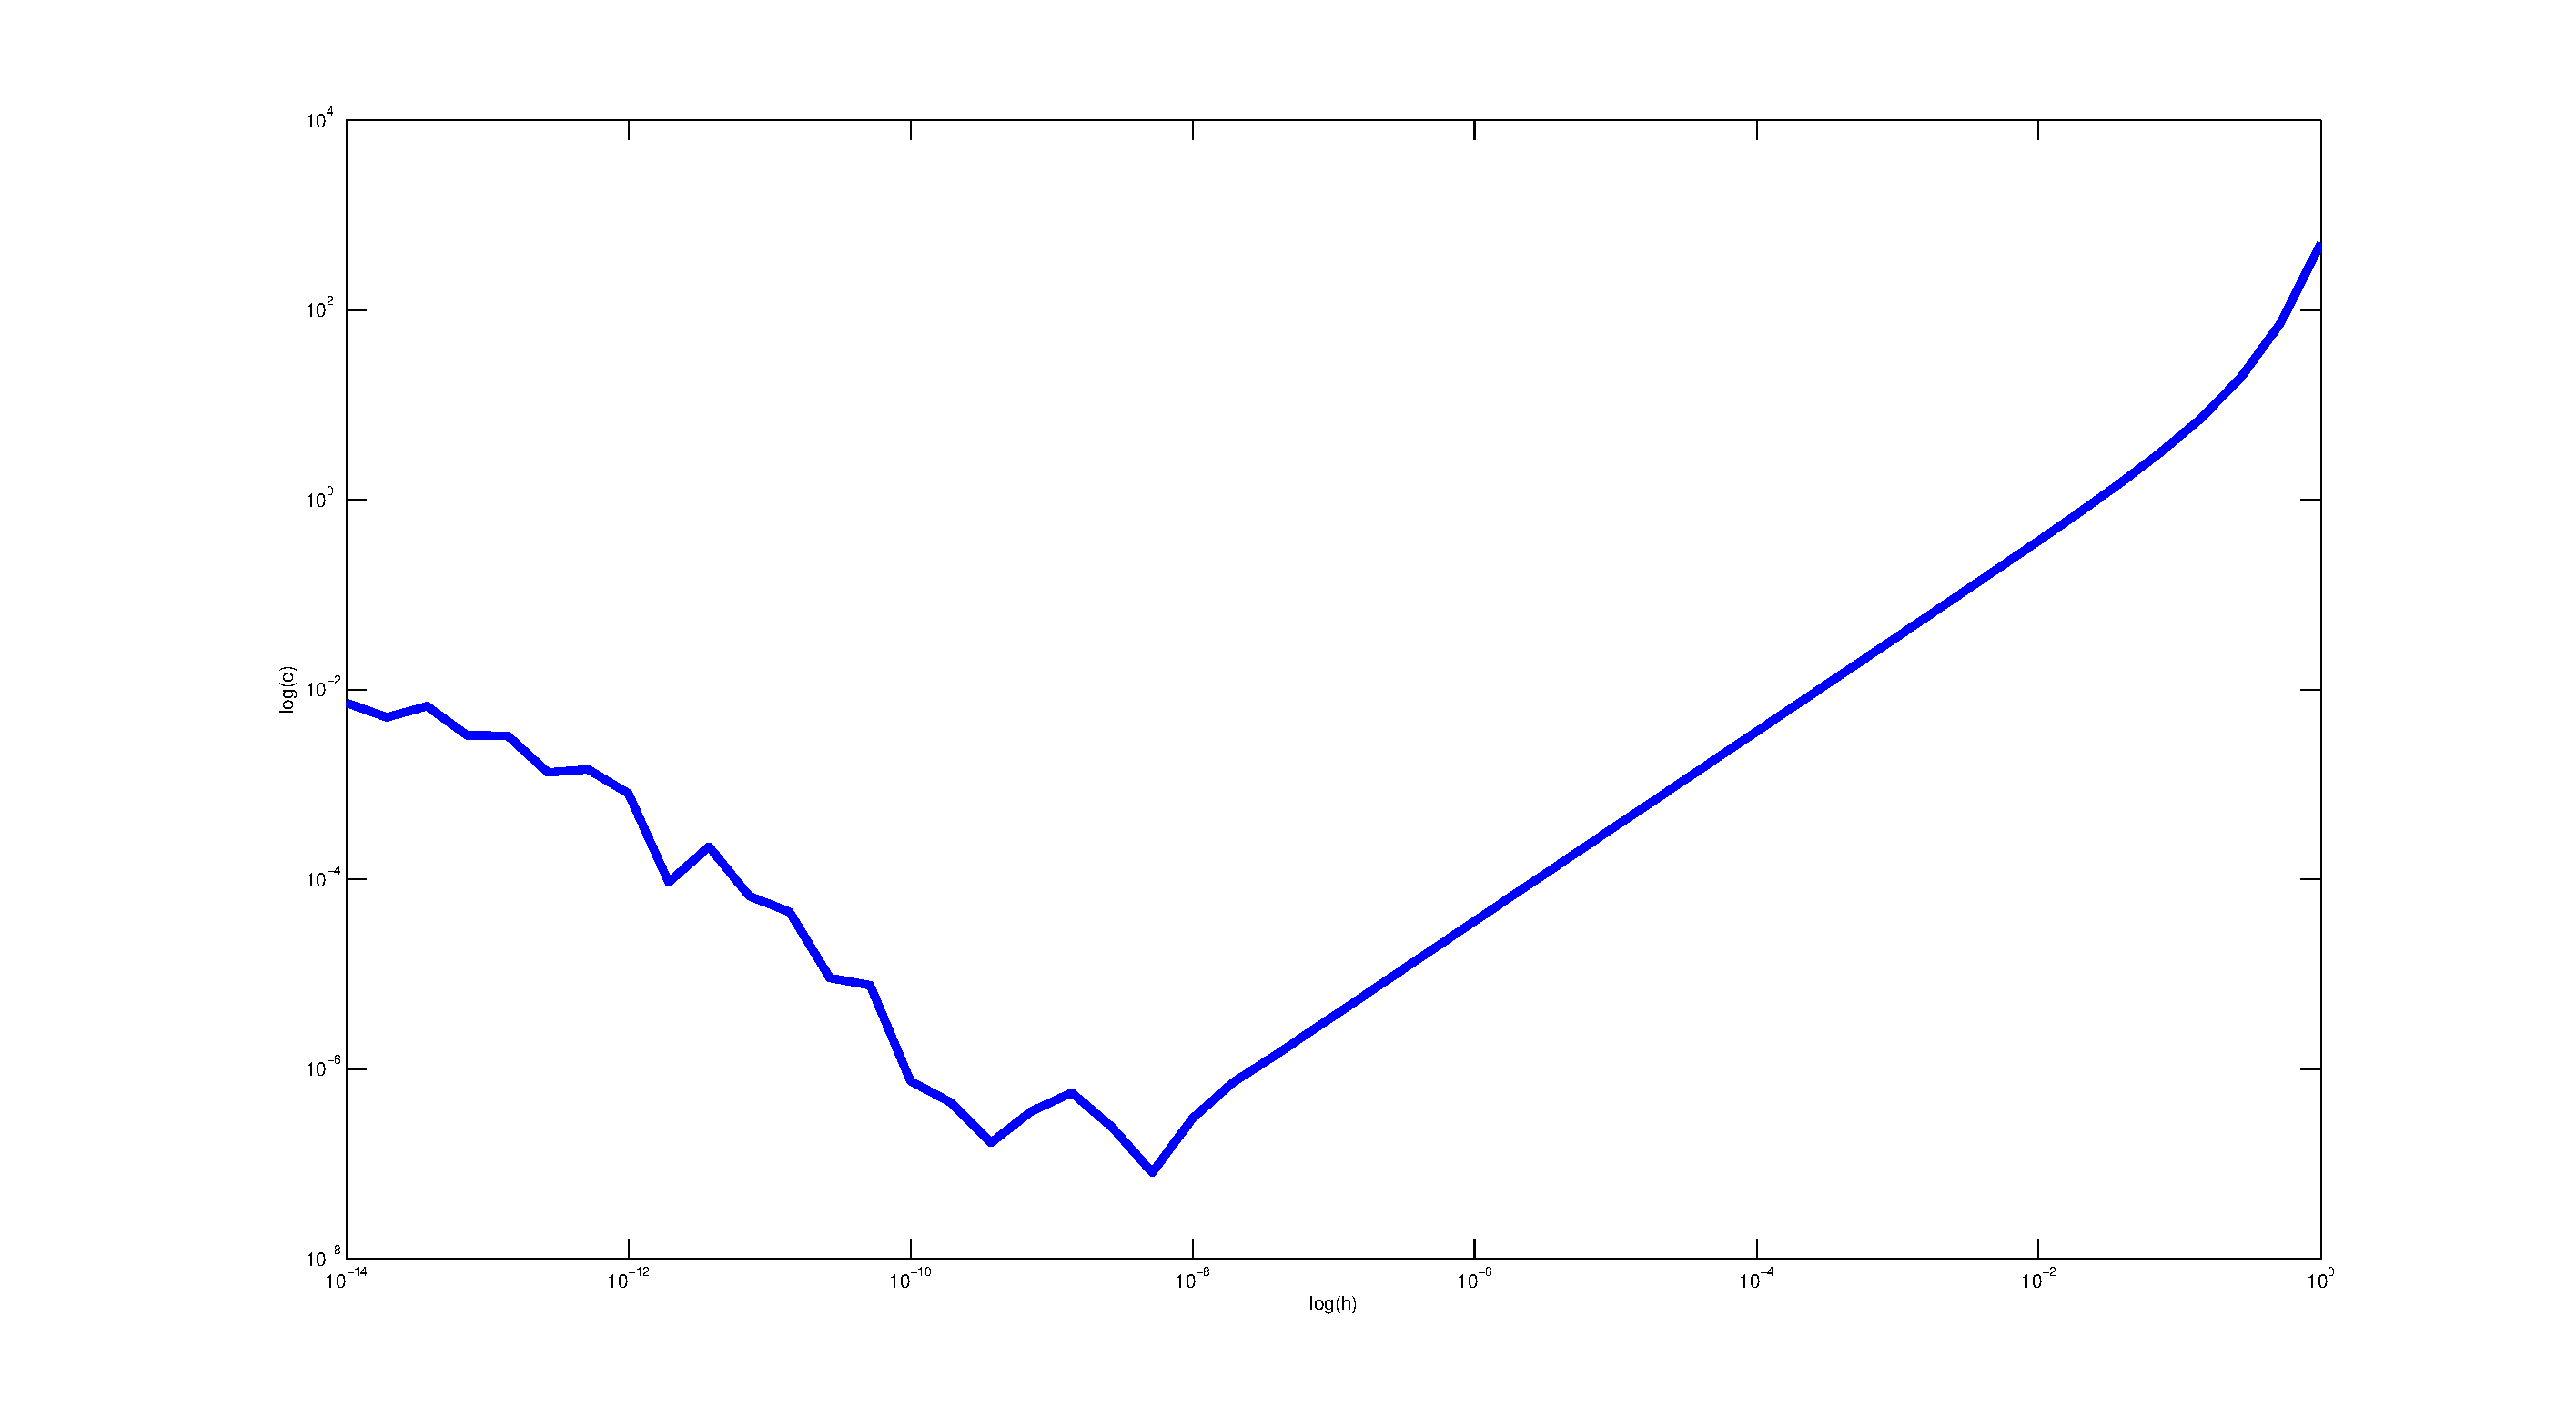
\includegraphics[scale=0.25]{ejem1.eps}
      \caption{Aproximaci\'on de $f'(1)$ para $f(x)=x^9$.}
    \end{figure}
  \end{center}
\end{frame}
%%%%%
\begin{frame}{Diferenciaci\'on Num\'erica}
  Se puede ver que los errores disminuyen hasta un cierto valor cr\'itico $h_{min}$ luego del cual los errores aumentan seg\'un la $h$ disminuye. \textquestiondown Contradice esto el resultado de arriba de $O(h)$ del error?
  \begin{itemize}
    \item<2-> El resultado anterior es sobre la convergencia si la aritm\'etica es exacta y se dice que es un resultado asint\'otico.
    \item<3-> La figura ilustra los efectos de redondeo debido a la aritm\'etica finita, los cuales se hacen significativos para $h$ peque\~no y pueden afectar cualquier f\'ormula num\'erica para aproximar la derivada.
  \end{itemize}
\end{frame}
%%%%%
\begin{frame}{Diferenciaci\'on Num\'erica}
  \begin{block}{Definici\'on:}
    El error de truncamiento se define como:
    $$
    E = |Du(x) - u'(x)|
    $$
    donde $u'(x)$ es la derivada y $Du(x)$ es su aproximaci\'on. Adem\'as, si $E \leq Ch^p$, se dice que el esquema $Du(x)$ tiene un orden de precisi\'on $p$, $O(h^p)$, siempre que $C$ sea una constante, la cual usualmente depende
    de la regularidad de $u(x)$.
  \end{block}
\end{frame}
%%%%%
\begin{frame}{Diferenciaci\'on Num\'erica}
  \begin{itemize}
    \item Una f\'ormula con un grado de aproximaci\'on digamos $O(h^2)$ es preferible a una de $O(h)$
    \item<2-> ya que los errores (te\'oricos) tienden a cero m\'as r\'apido y as\'i la $h$ no se tiene que hacerse tan peque\~na reduciendo as\'i los efectos de los errores por la aritm\'etica finita.
    \item<3-> Es posible, mejorar la precisi\'on de la siguiente manera: Sean los polinomios de Taylor de las funciones $f(x_0 + h)$ y $f(x_0 - h)$, suponiendo que la funci\'on es al menos tres veces derivable:
    \begin{align*}
    f(x_0+h) &= f(x_0) + f'(x_0)h + \dfrac{f''(x_0)}{2}h^2 + \dfrac{f'''(\xi_1)}{6}h^3\\
    f(x_0-h) &= f(x_0) - f'(x_0)h + \dfrac{f''(x_0)}{2}h^2 - \dfrac{f'''(\xi_2)}{6}h^3
    \end{align*}
  \end{itemize}
\end{frame}
%%%%%
\begin{frame}{Diferenciaci\'on Num\'erica}
  \begin{itemize}
    \item Restando ambas ecuaciones y resolviendo para $f'(x_0)$:
    $$
    f'(x_0) = \dfrac{f(x_0+h)-f(x_0-h)}{2h} - \dfrac{h^2}{12}(f'''(\xi_1)+f'''(\xi_2))
    $$
    \item<2-> Como $f \in \mathcal{C}^3 [x_0-h, x_0+h]$, entonces por el teorema del valor intermedio existe $\xi \in [x_0-h, x_0+h]$ tal que,
    $$
    f'''(\xi) = \dfrac{f'''(\xi_1)+f'''(\xi_2)}{2}
    $$   
  \end{itemize}
\end{frame}
%%%%%
\begin{frame}{Diferenciaci\'on Num\'erica}
  \begin{itemize}
    \item Por lo anterior queda entonces que:
    $$
    f'(x_0) = \dfrac{f(x_0+h)-f(x_0-h)}{2h} - \dfrac{f'''(\xi)}{6}h^2
    $$
    \item<2-> A esta expresi\'on se le llama f\'ormula de diferencia centrada, el orden de precisi\'on es 2, mientras que el error de truncamiento es $O(h^2)$.
    \end{itemize}
\end{frame}
%%%%
\begin{frame}{Diferenciaci\'on Num\'erica}
\begin{center}
 \begin{figure}
 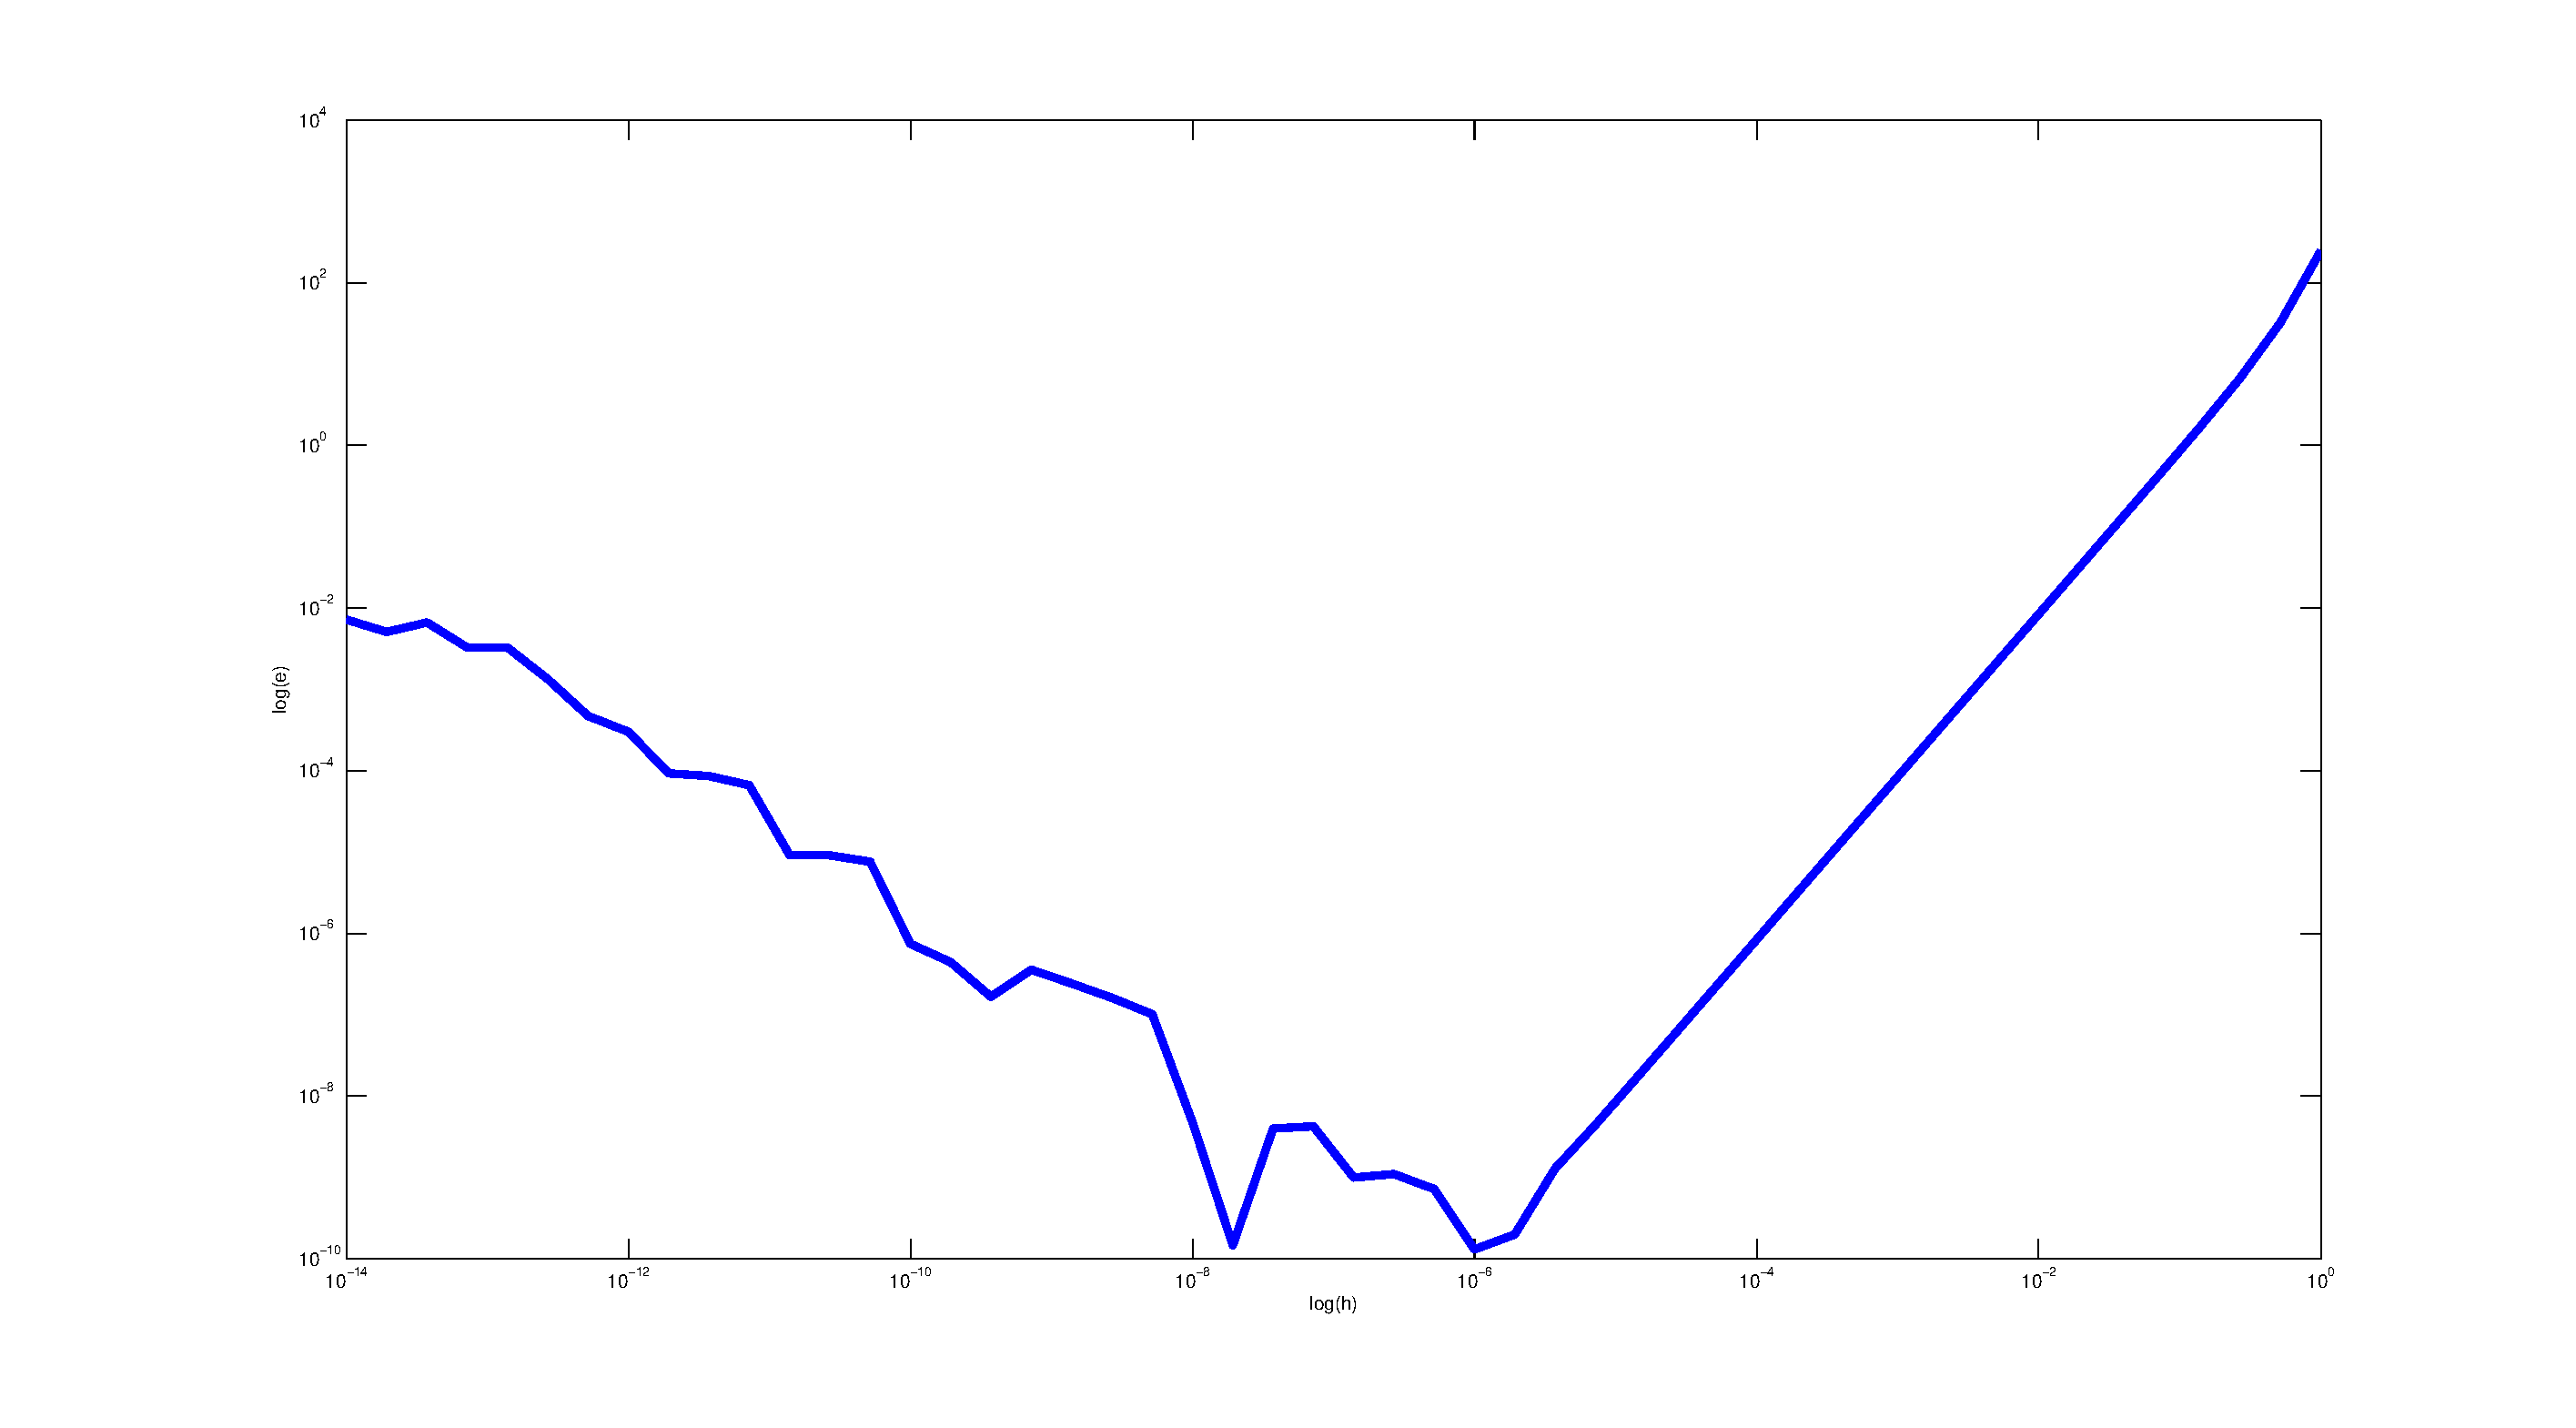
\includegraphics[scale=0.25]{ejem2.eps}
 \caption{Aproximaci\'on de $f'(1)$ para $f(x)=x^9$.}
\end{figure}
\end{center}
\end{frame}
%%%%%
\begin{frame}{F\'ormula de los $n$ puntos.}
El siguiente teorema utiliza el polinomio interpolador de una funci\'on $f$ para obtener f\'ormulas de aproximaci\'on a la derivada de una funci\'on $f$.
\uncover<2->{
\begin{block}{Teorema 1 (f\'ormula de $n$ puntos)}
Sea $f$ una funci\'on de clase $C^{n+1} [a, b]$ y $\{x_1,x_2,\ldots,x_n\}$ $n$ puntos distintos de dicho intervalo. Si llamamos $L_i(x)$ a los correspondientes polinomios elementales de Lagrange de grado $n-1$, entonces existe un punto $\xi \in [a,b]$ tal que
$$
f'(x_k) = \sum_{i=1}^nf(x_i)L'_i(x_k) + \frac{f^{(n)}(\xi)}{n!}\prod_{i=1,i\neq k}^n(x_k-x_i)
$$
\end{block}}
\end{frame}+
%%%%
\begin{frame}{F\'ormula de los $n$ puntos.}
  \begin{itemize}
    \item El polinomio de segundo grado que interpola a $f$ en los puntos $x_0,x_1,x_2$, tiene por polinomios elementales:
  \end{itemize}
\begin{align*}
\uncover<2->{L_0(x) = \frac{(x-x_1)(x-x_2)}{(x_0-x_1)(x_0-x_2)} & \Rightarrow L'_0(x) = \frac{(x-x_2)+(x-x_1)}{(x_0-x_1)(x_0-x_2)}\\}
\uncover<3->{L_1(x) = \frac{(x-x_0)(x-x_2)}{(x_1-x_0)(x_1-x_2)} & \Rightarrow L'_1(x) = \frac{(x-x_2)+(x-x_0)}{(x_1-x_0)(x_1-x_2)}\\}
\uncover<4->{L_2(x) = \frac{(x-x_0)(x-x_1)}{(x_2-x_0)(x_2-x_1)} & \Rightarrow L'_2(x) = \frac{(x-x_1)+(x-x_0)}{(x_2-x_0)(x_2-x_1)}}
\end{align*}
\end{frame}
%%%%
\begin{frame}{F\'ormula de los $n$ puntos}
  \begin{itemize}
    \item De esta manera, siguiendo el teorema anterior, se tendr\'ia que:
    {\footnotesize
      \begin{align*}
f'(x_k) &= \frac{f(x_0)[(x_k-x_2)+(x_k-x_1)]}{(x_0-x_1)(x_0-x_2)} + \frac{f(x_1)[(x_k-x_2)+(x_k-x_0)]}{(x_1-x_0)(x_1-x_2)}\\
 & + \frac{f(x_2)[(x_k-x_1)+(x_k-x_0)]}{(x_2-x_0)(x_2-x_1)} + \frac{f'''(\xi)}{3!}\prod_{i=0,i\neq k}^2(x_k-x_i)\\
& \qquad\qquad\qquad\qquad\qquad\qquad\qquad\qquad\qquad\forall k=0,1,2
\end{align*}}
    \end{itemize}
\end{frame}
%%%%
\begin{frame}{F\'ormula centrada de tres puntos.}
Si tomamos $x_0 = x_1-h$, $x_1 = x_1$ y $x_2 = x_1 + h$ para aproximar $f'(x_1)$, nos queda que:
\begin{align*}
f'(x_1) =&  \frac{f(x_0)(x_1-x_2)}{(x_0-x_1)(x_0-x_2)} + \frac{f(x_1)[(x_1-x_2)+(x_1-x_0)]}{(x_1-x_0)(x_1-x_2)}\\
 &+ \frac{f(x_2)(x_1-x_0)}{(x_2-x_0)(x_2-x_1)} + \frac{f'''(\xi)}{3!}\prod_{i=0,i\neq 1}^2(x_1-x_i)
\end{align*}
\uncover<2->{Sustituyendo $x_0$ y $x_2$, y simplificando la expresi\'on se obtiene:
\begin{align*}
f'(x_1) & = \frac{f(x_1+h)-f(x_1-h)}{2h} - \frac{f'''(\xi)}{6}h^2
\end{align*}}
\end{frame}
%%%%
\begin{frame}{F\'ormula progresiva de tres puntos.}
Si tomamos $x_0 = x_0$, $x_1 = x_0+h$ y $x_2 = x_0 + 2h$ para aproximar $f'(x_0)$ con $h > 0$ , queda que:
\begin{align*}
f'(x_0) &=  \frac{f(x_0)[(x_0-x_2)+(x_0-x_1)]}{(x_0-x_1)(x_0-x_2)} + \frac{f(x_1)(x_0-x_2)}{(x_1-x_0)(x_1-x_2)}\\
& + \frac{f(x_2)(x_0-x_1)}{(x_2-x_0)(x_2-x_1)} + \frac{f'''(\xi)}{3!}\prod_{i=0,i\neq 0}^2(x_0-x_i)
\end{align*}
\uncover<2->{Sustituyendo $x_1$ y $x_2$, y simplificando la expresi\'on se obtiene:
\begin{align*}
f'(x_0) & = \frac{-3f(x_0)+4f(x_0+h)-f(x_0+2h)}{2h} + \frac{f'''(\xi)}{3}h^2\nonumber
\end{align*}}
\end{frame}
%%%%
\begin{frame}{F\'ormula regresiva de tres puntos.}
Si tomamos $x_0 = x_2-2h$, $x_1 = x_2-h$ y $x_2 = x_2$ para aproximar $f'(x_2)$ con $h > 0$ , queda que:
\begin{align*}
f'(x_2) &=  \frac{f(x_0)(x_2-x_1)}{(x_0-x_1)(x_0-x_2)} + \frac{f(x_1)(x_2-x_0)}{(x_1-x_0)(x_1-x_2)}\\
 &+ \frac{f(x_2)[(x_2-x_1)+(x_2-x_0)]}{(x_2-x_0)(x_2-x_1)} + \frac{f'''(\xi)}{3!}\prod_{i=0,i\neq 2}^2(x_2-x_i)
\end{align*}
\uncover<2->{Sustituyendo $x_0$ y $x_1$, y simplificando la expresi\'on se obtiene:
\begin{align*}
f'(x_2) & = \frac{f(x_2-2h)-4f(x_2-h)+3f(x_2)}{2h} + \frac{f'''(\xi)}{3}h^2\nonumber
\end{align*}}
\end{frame}
%%%%
\begin{frame}{Derivadas de Orden Superior}
  \begin{itemize}
    \item A partir del desarrollo de Taylor de la funci\'on evaluada en $x_0 + h$ y $x_0 - h$, se puede
    obtener la f\'ormula para la que aproxima a la segunda derivada de la funci\'on $f$.
    \item<2-> Sea $0<|h|<\delta$ por Taylor, suponiendo que $f^{(4)}$ existe y es continua en $(x_0-\delta,x_0+\delta)$, $\xi_1$ entre $x_0$ y $x_0+h$, $\xi_2$ entre $x_0$ y $x_0-h$.
  \end{itemize}
  \uncover<3->{
  \begin{align*}
    f(x_0+h) &= f(x_0) + f'(x_0)h + \dfrac{f''(x_0)}{2}h^2 + \dfrac{f'''(x_0)}{6}h^3 + \dfrac{f^{(4)}(\xi_1)}{24}h^4\\
    f(x_0-h) &= f(x_0) - f'(x_0)h + \dfrac{f''(x_0)}{2}h^2 - \dfrac{f'''(x_0)}{6}h^3 + \dfrac{f^{(4)}(\xi_2)}{24}h^4
  \end{align*}}
\end{frame}
%%%%
\begin{frame}{Derivadas de Orden Superior}
  \begin{itemize}
    \item Sumandos ambas ecuaciones:
    {\small
    $$
     f(x_0+h) + f(x_0-h) = 2f(x_0) +2\dfrac{f''(x_0)}{2}h^2 + \dfrac{h^4}{24}\left(f^{(4)}(\xi_1)+f^{(4)}(\xi_2)\right)
     $$}
     \item y despejando $f''(x_0)$ de esta expresi\'on se obtiene:     
     $$
     f''(x_0) = \dfrac{f(x_0+h) - 2f(x_0) + f(x_0-h)}{h^2} + \dfrac{f^{(4)}(\xi)}{12}h^2 
    $$
    con $\xi \in (x_0-h,x_0+h)$
  \end{itemize}
\end{frame}
%%%%%
\section{Integraci\'on Num\'erica}
\begin{frame}{Tema 2}
    \begin{itemize}
        \item Contenido del tema 2
        \item Explicación $a$
    \end{itemize}
\end{frame}
\end{document}

